\usepackage{float}

\section{Design}
\label{sec:design}

\subsection{Use Cases}
The use cases of the Feed App are quite simple in nature and do not require a large amount of explanation. However, before we dig into the details of the use cases, it is important to note that certain functionalities are locked to whether you are a registered user or not.

\subsubsection{Create Poll}
This part lets registered users create polls consisting of:
\begin{itemize}
    \item \textbf{PollID}: An automatically generated identifier for the polls that is used for request-logic such as updating, getting, and deleting the poll later on.
    \item \textbf{Title/Question}: This is the question that the registered user wants to ask the voters.
    \item \textbf{Options}: These consist of all the options that the creator wants to give the voters to vote on.
\end{itemize}

\subsubsection{Vote on Poll}
When it comes to voting on polls, it is restricted to registered users only, and therefore anyone who wants to vote will have to create an account in the app. The polls that the users vote on will consist of a question, and then the voting options accompanied by the current amount of votes. 

There is, however, a discussion to be made around whether or not the current votes should be public before making a vote, as this can sway the user into voting something that they might not have otherwise. On the other hand, having the votes public from the start will make sure that everything is transparent for the voters and also keep them as informed as possible.

\subsubsection{See Poll}
For the visibility of the polls on the website, there was no real reason to gatekeep what the available polls on the site look like. Therefore, both registered and unregistered users can see and read the polls that have been created by the registered users.

\subsubsection{Create Account}
Creating an account is an action that is required to do in order to create and vote on polls on the app. The act of creating an account requires the unregistered user to put in their login details that will consist of a name, password, and email.

\subsubsection{Log into Account}
For the last use case, there is the functionality of logging into the created accounts. This simply requires the registered user to type in the details used to create their account, and they will then be fully logged in and ready to use all the functionalities that the app has to offer in the UI.

\begin{figure}[thb]
	\centering
	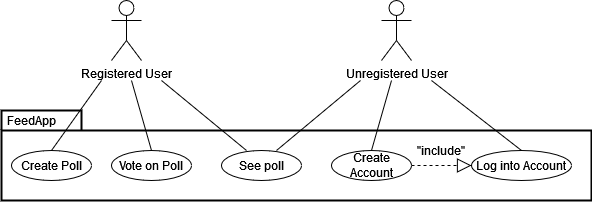
\includegraphics[scale=0.5]{figs/usecases.png}
	\caption{Use cases of the FeedApp.}
	\label{fig:usecases}
\end{figure}

\subsection{Domain Model}
This section will describe the domain model.

\begin{figure}[thb]
	\centering
	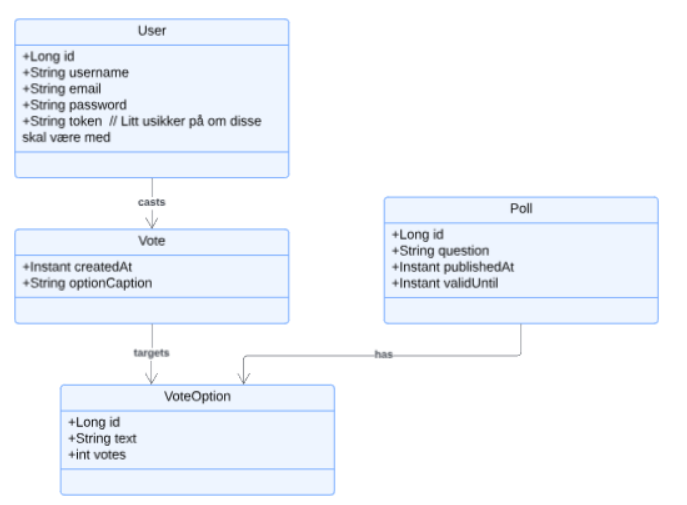
\includegraphics[scale=0.5]{figs/domainmodel.png}
	\caption{Domain model of the FeedApp.}
	\label{fig:domainmodel}
\end{figure}

\subsection{Entities and Attributes}

\subsubsection{Poll}
A \textbf{Poll} represents the central object of the application, allowing users to create questions with a specified validity period. It contains the following attributes:
\begin{itemize}
    \item \textbf{id:} A unique identifier for the poll (Long).
    \item \textbf{question:} The main question posed in the poll (String).
    \item \textbf{publishedAt:} The timestamp when the poll was published (Instant).
    \item \textbf{validUntil:} The expiration timestamp of the poll (Instant).
\end{itemize}
Each poll is associated with multiple \textbf{VoteOption} objects, which represent the possible answers users can vote on.

\subsubsection{VoteOption}
A \textbf{VoteOption} represents a single selectable option in a poll. It includes:
\begin{itemize}
    \item \textbf{id:} A unique identifier for the option (Long).
    \item \textbf{text:} The text description of the voting option (String).
    \item \textbf{votes:} The number of votes this option has received (int).
\end{itemize}
Each \textbf{VoteOption} belongs to a \textbf{Poll} and is updated as users cast their votes.

\subsubsection{Vote}
A \textbf{Vote} captures a user's action when selecting an option in a poll. It contains:
\begin{itemize}
    \item \textbf{createdAt:} The timestamp when the vote was cast (Instant).
    \item \textbf{optionCaption:} A reference to the selected voting option's text (String).
\end{itemize}
The \textbf{Vote} is linked to a specific \textbf{User} and a specific \textbf{VoteOption} within a \textbf{Poll}.

\subsubsection{User}
The \textbf{User} entity represents individuals interacting with the application, whether to create polls, vote, or view analytics. Attributes include:
\begin{itemize}
    \item \textbf{id:} A unique identifier for the user (Long).
    \item \textbf{username:} The display name of the user (String).
    \item \textbf{email:} The user’s email address (String).
\end{itemize}
Additional attributes such as \textit{password} and \textit{token} were considered but remain undecided for inclusion due to potential security concerns and implementation details.

\subsection{Relationships}
\begin{itemize}
    \item A \textbf{Poll} has multiple \textbf{VoteOptions}, forming a one-to-many relationship.
    \item A \textbf{User} casts multiple \textbf{Votes}, establishing a one-to-many relationship.
    \item Each \textbf{Vote} targets a single \textbf{VoteOption} within a specific \textbf{Poll}, creating a many-to-one relationship.
\end{itemize}

\subsection{Discussion}
The current domain model supports the core functionalities of the application, including poll creation, voting, and analytics generation. The use of \texttt{Instant} for timestamps ensures precise time tracking, which is critical for enforcing poll validity and generating accurate analytics. The relationships between entities provide a scalable and flexible structure to accommodate additional features in the future.

The model's simplicity ensures ease of implementation while maintaining the necessary complexity to meet the application requirements.

\subsection{Architecture}

\subsubsection{Web UI / Elm}
The web UI of the feed app is also the featured technology of this project. Therefore, it will be covered later on in a more in-depth look into the implementation and choice of the Elm programming language as our frontend framework for our web UI.

\subsubsection{REST API / Spring Web MVC}
The REST API works as the middleman between the frontend and backend as a way to perform all the CRUD operations in the application. This means that the integration of the REST API allows us to POST, UPDATE, GET, and DELETE data about the users and polls.

When it comes to the choice of using Spring Web MVC to implement this, there was not any good reason for us to change as the entire team has experience using it, and it also works seamlessly with the rest of the stack, as the Spring Web MVC is a dependency from the Spring Framework, which also has dependencies for Java, JPA, H2, RabbitMQ, and MongoDB. 

\subsubsection{Business Logic / Java}
For the business logic part of the project, we chose to go with Java for the simple reasons of reliability, familiarity, and possibilities. In other words, the entire group has experience working with Java, and the language gives us everything we need to create the feed app that we want. It also integrates well with the other components of the app, for example through the use of Spring Framework.

Alternatives would be to go the same route as mentioned in the section about alternatives for REST API, in other words the alternatives were other big enterprise languages such as Python, JavaScript, Ruby, and Kotlin. 

\subsubsection{Persistence \& Relational Database / JPA \& H2}
JPA (Java Persistence API) is the technology that connects our business logic with our relational database, which in this case is H2. JPA makes it possible to map Java objects to database tables, and it also allows us to do CRUD operations directly on our Java objects. 

The reason that the group went with JPA is that it also has a dependency and operability with Spring Framework, which makes it integrate easily and just work really well with the rest of our chosen stack.

When it comes to the choice of H2 for our database, it also works really easily and well because of its integration with the Spring Framework. In addition, it is a very simple and easy-to-learn database that gives us everything we need. One of the reasons we didn't need to go for any more complex databases, is that we also have an analytics component that gives us insight into the app’s data through its use of MongoDB as a non-relational database.

\subsubsection{Message Broker / RabbitMQ}
The message broker is one of the two parts that make up the analytics component of the project. The purpose of this message broker is to give us asynchronous communication between the feed app (business logic) and the database in the analytics component, which means that we don’t need real-time conversation to have interaction between the app and the analytics component. 

The positive side of doing this is that no messages will be lost, and that they are processed in the order they are sent by message queues in RabbitMQ. Message queues are simply a message that is stored for an indefinite time until it is processed, and then deleted from the queue.

The reason we chose RabbitMQ for message handling is that it supports the publish/subscribe model that we wanted to implement in our feed app, and it is also supported in Spring Framework through Spring AMQP, which makes it integrate very well with the rest of the stack.

Alternatives that we looked at were Apache Kafka and Redis, however they either provided too much unnecessary complexity (Kafka) or didn't offer the robustness that we needed (i.e Redis didn’t offer automatic re-delivery). Also the group had experience using RabbitMQ from earlier, so there was no real incentive to go for anything other than RabbitMQ, as it provided us all the functionality and ease-of-use that we needed for a message broker.

\subsubsection{Non-relational Database / MongoDB}
The non-relational database is the second part of the application’s analytics component, and is used to store all the data in an analytics-collection. This is then used to understand voting patterns, typical questions, and can be used to just learn more about the users of the feed app in general.

When it comes to the choice of MongoDB as the database, it was not a straightforward choice. We also had a serious look at Apache Cassandra and even possibly using Redis as the non-relational database. Both of these offered perks that we could not get with MongoDB, such as Apache Cassandra offering really good scalability and working very well with big data. Redis on the other hand can be used as a very lightweight and high-speed database that stores data in memory and also has built-in pub/sub functionality (meaning it can be used as both a message broker AND non-relational database), which makes it very easy and beginner-friendly to implement. Even though these two alternatives provide some good perks of use, there are still good reasons to pick MongoDB over them, and also it provides sort of a middle ground between Cassandra and Redis. The reason we decided to go for MongoDB was that it works for everything we need, which is to view our analytics in a simple document-model. It gives us a simplicity and ease-of-use that Cassandra cannot deliver, and also it lets us view our analytics in a way that Redis cannot deliver as easily (for example the use of complex queries like “find()” from MongoDB is not provided in Redis).

\begin{figure}[H]
	\centering
	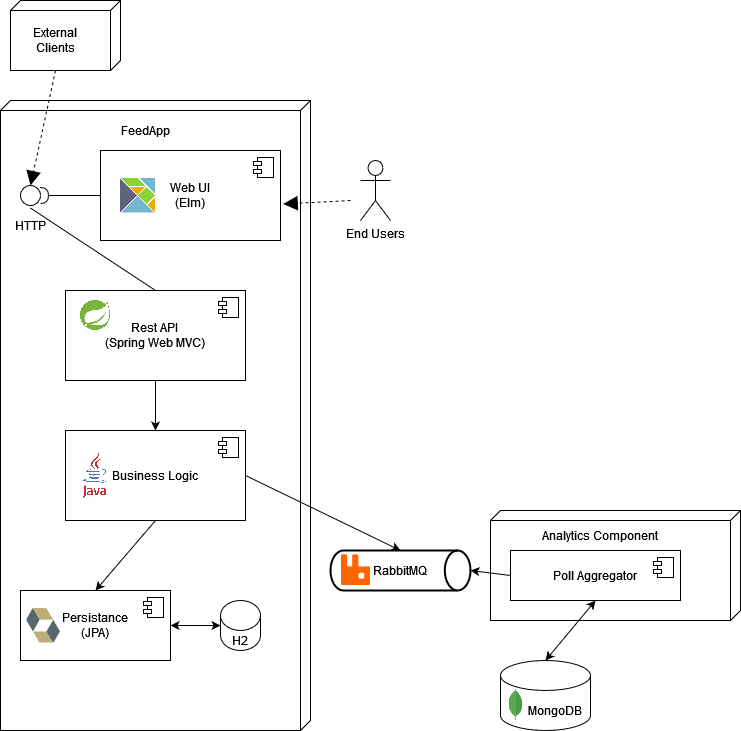
\includegraphics[scale=0.5]{figs/DAT250architecture.png}
	\caption{The software architecture of the FeedApp.}
	\label{fig:DAT250architecture}
\end{figure}
